\documentclass[10pt, oneside]{article}
\usepackage[a4paper, total={5.5in, 9in}]{geometry}
\usepackage[ngerman]{babel}

\usepackage{blindtext}
\usepackage{titlesec}
\usepackage{amsmath}
\usepackage[hidelinks]{hyperref}
\usepackage{parskip}
\usepackage{graphicx}
\usepackage{longtable}
\usepackage[shortlabels]{enumitem}
\usepackage{multirow}
\usepackage{nccmath}
\usepackage{rotating}
\usepackage{makecell}
\usepackage{multicol}
\usepackage{capt-of}
\usepackage{csquotes}
\usepackage{amsfonts}
\usepackage{caption}

\captionsetup[table]{position=bottom}

\titleformat{\section}
    {\normalfont\Large\bfseries}{}{0pt}{}

\let\oldsection\section
\renewcommand{\section}{
  \renewcommand{\theequation}{\thesection.\arabic{equation}}
  \oldsection}
\let\oldsubsection\subsection
\renewcommand{\subsection}{
  \renewcommand{\theequation}{\thesubsection.\arabic{equation}}
  \oldsubsection}

\makeatletter
\renewcommand{\maketitle}{
    \bgroup
    \centering
    \par\LARGE\@title  \\[20pt]
    \par\large\@author \\[10pt]
    \par\large\@date
    \par
    \egroup
}
\makeatother


\title{Technische Informatik\\[10pt]\Large{WiSe 2024/25}\\[15pt]\Large{L{\"o}sungen zum {\"U}bungsblatt 6}}
\author{Volodymyr But\\[10pt]Hochschule Trier}
\date{}

% - - - - - - - - - - - - - - - - - - - - - - - - - - - - - - - - - - - - - - %

\begin{document}

\maketitle
\vspace{25px}

\setcounter{section}{2}
\section{Aufgabe 3}

Bestimmen Sie die Werte von $A, B, C$ und $D$ so, dass
\begin{enumerate}[(a)]
    \item $A + \overline{B} + C + \overline{D} = 0$ : $A = 0$, $B = 1$, $C = 0$, $D = 1$
    \item $A \cdot \overline{B} \cdot C \cdot \overline{D} = 0$ : $A = 1$, $B = 0$, $C = 1$, $D = 0$
    \item $\overline{A} \cdot \overline{B} = 0$ : $A = 0$, $B = 0$
\end{enumerate}

\section{Aufgabe 4}

Beweisen Sie die G"ultigkeit der Gliechung $A + A \cdot B = A$.
\begin{align*}
    A + A \cdot B &= A \\
    A \cdot 1 + A \cdot B &= A \\
    A \cdot (1 + B) &= A \\
    A \cdot 1 &= A \\
    A &= A \quad \text{\underline{q.e.d.}}
\end{align*}

\section{Aufgabe 5}

Leiten Sie mit Hilfe der bekannten algebraischen Regeln die G¨ultigkeit der gegebenen
Gleichung $A + \overline{A} \cdot B = A \cdot B$ her.
\begin{align*}
    A + \overline{A} \cdot B &= A + B \\
    A + A \cdot B + \overline{A} \cdot B &= A + B \\
    A + B \cdot (A + \overline{A}) &= A + B \\
    A + B \cdot 1 &= A + B \\
    A + B &= A + B \quad \text{\underline{q.e.d.}}
\end{align*}

\pagebreak
\section{Aufgabe 6}

In der Booleschen Algebra wird oft ein zweites Distributivgesetz angegeben:
\begin{equation*}
    (A + B) \cdot (C + D) = A \cdot C + A \cdot D + B \cdot C + B \cdot D
\end{equation*}
Leiten Sie dieses aus dem Ihnen bekannten Distributivgesetz her.
\begin{align*}
    (A + B) \cdot (C + D)                         &= A \cdot C + A \cdot D + B \cdot C + B \cdot D \\
    (A + B) \cdot C + (A + B) \cdot D             &= A \cdot C + A \cdot D + B \cdot C + B \cdot D \\
    (AC + BC) + (AD + BD)                         &= A \cdot C + A \cdot D + B \cdot C + B \cdot D \\
    A \cdot C + A \cdot D + B \cdot C + B \cdot D &= A \cdot C + A \cdot D + B \cdot C + B \cdot D \quad \text{\underline{q.e.d.}}
\end{align*}

\section{Aufgabe 7}

Leiten Sie mit Hilfe der bekannten algebraischen Regeln die G"ultigkeit der
gegebenen Gleichung her.
\begin{align*}
    (A + B) \cdot (A + C) &= A + B \cdot C \\
    AA + AC + BA + BC &= A + B \cdot C \\
    A + AC + BA + BC &= A + B \cdot C \\
    A + AB + BC &= A + B \cdot C \\
    A + B \cdot C &= A + B \cdot C \quad \text{\underline{q.e.d.}}
\end{align*}

\section{Aufgabe 8}

Stellen Sie anhand der gegebenen Schaltung die logische Gleichung f"ur $Q$ auf.
\begin{figure*}[h]
    \centering
    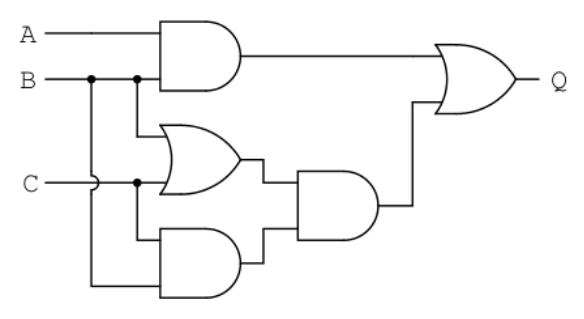
\includegraphics[scale=0.3]{./8.png}
\end{figure*}

\begin{align*}
    AB + ((B + C) \cdot BC) &= AB + BBC + BCC = \\
                            &= AB + BC + BC \\
                            &= AB + BC = \\
                            &= B(A + C)
\end{align*}
\begin{figure*}[h]
    \centering
    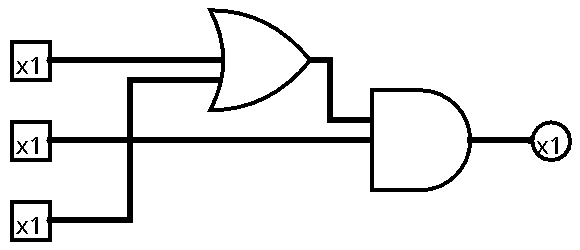
\includegraphics[scale=0.25]{./8-1.png}
\end{figure*}

\section{Aufgabe 9}
\begin{enumerate}[(a)]
    \item Verwenden Sie die Regeln der Booleschen Algebra zur Vereinfachung des
        Booleschen Ausdrucks:
        \begin{align*}
            A \cdot B + A \cdot (B + C) + B \cdot (B + C) &= AB + AB + AC + BB + BC = \\
                                                          &= AB + AC + B + BC = \\
                                                          &= AB + AC + B = \\
                                                          &= B + AC
        \end{align*}
    \item Zeichnen Sie die logischen Schaltkreise f"ur den optimierten Ausdruck.
        \begin{figure*}[h]
            \centering
            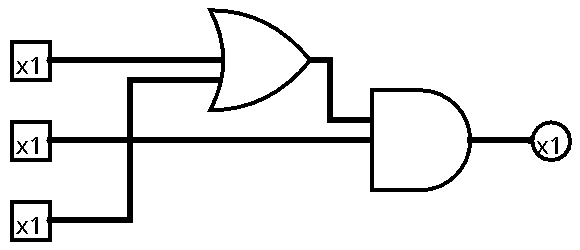
\includegraphics[scale=0.25]{./8-1.png}
        \end{figure*}
\end{enumerate}

\section{Aufgabe 10}

Verwenden Sie die Regeln der Booleschen Algebra zur Vereinfachung der
Booleschen Ausdr"ucke.

\begin{enumerate}[(a)]
    \item $\begin{aligned}[t]
               &[A \cdot \overline{B} \cdot (C + B \cdot D) + \overline{A} \cdot \overline{B}] \cdot C = \\
            =\ &[A \cdot \overline{B} \cdot C + A \cdot \overline{B} \cdot B \cdot D) + \overline{A} \cdot \overline{B}] \cdot C = \\
            =\ &[A \cdot \overline{B} + 0 + \overline{A} \cdot \overline{B}] \cdot C = \\
            =\ &A \cdot \overline{B} \cdot C + \overline{A} \cdot \overline{B} \cdot C = \\
            =\ &\overline{B}C(A + \overline{A}) = \\
            =\ &\overline{B}C
        \end{aligned}$
    \item $\begin{aligned}[t]
            A \cdot (A + B) = AA + AB = A + AB = A
        \end{aligned}$
    \item $\begin{aligned}[t]
            A \cdot (\overline{A} + A \cdot B) = A\overline{A} + AAB = 0 + AB = AB
        \end{aligned}$
    \item $\begin{aligned}[t]
            B \cdot C + \overline{B} \cdot C = C \cdot (B + \overline{B}) = C
        \end{aligned}$
\end{enumerate}

\section{Aufgabe 11}

Bestimmen Sie den logischen Ausdruck f"ur die Schaltung in der Aufgabensammlung:
\begin{align*}
       &(C \cdot \overline{D} \cdot \overline{B}) + (A \cdot \overline{B})
\end{align*}

\section{Aufgabe 12}

Wandeln Sie die Terme mit DeMorgans Theoremen um, so dass jede Variable nur
noch an maximal einer Negation beteiligt ist; also jedes Vorkommen jeder
Variablen unter maximal einem Strich steht.
\begin{enumerate}[(a)]
    \item $\begin{aligned}[t]
            \overline{\overline{(X \cdot \overline{Y})} \cdot (\overline{Y} + Z)} &= \overline{\overline{(X \cdot \overline{Y})}} + \overline{(\overline{Y} + Z)} = \\
                                                                                  &= (X \cdot \overline{Y}) + (Y \cdot \overline{Z})
        \end{aligned}$
    \item $\begin{aligned}[t]
            \overline{(\overline{X} + Z) \cdot \overline{(X \cdot Y)}} &= \overline{(\overline{X} + Z)} + \overline{\overline{(X \cdot Y)}} = \\
                                                                       &= (X \cdot \overline{Z}) + (X \cdot Y)
        \end{aligned}$
    \item $\begin{aligned}[t]
            \overline{\overline{A + B \cdot \overline{C}} + D \cdot (\overline{E + \overline{F}})} &= (A + B \cdot \overline{C}) \cdot (\overline{D} + (E + \overline{F}))
        \end{aligned}$
\end{enumerate}

\section{Aufgabe 13}

Wenden Sie DeMorgans Theoreme auf die folgenden Ausdr"ucke:
\begin{enumerate}[(a)]
    \item $\begin{aligned}[t]
            \overline{A + \overline{B}} = \overline{A} \cdot B
        \end{aligned}$
    \item $\begin{aligned}[t]
            \overline{\overline{A} \cdot B} = A + \overline{B}
        \end{aligned}$
    \item $\begin{aligned}[t]
            \overline{A + B + C} = \overline{A} \cdot \overline{B} \cdot \overline{C}
        \end{aligned}$
    \item $\begin{aligned}[t]
            \overline{A \cdot B \cdot C} = \overline{A} + \overline{B} + \overline{C}
        \end{aligned}$
\end{enumerate}

\section{Aufgabe 16}

Ermitteln Sie aus der gegebenen Wertetabelle (in der Aufgabensammlung)

\begin{enumerate}[(a)]
    \item einen $SOP$ Ausdruck:
        $\overline{A}BC + A\overline{B}\overline{C} + AB\overline{C} + ABC$
    \item einen $POS$ Ausdruck:
        $(A + B + C) \cdot (A + B + \overline{C}) \cdot (A + \overline{B} + C) \cdot (\overline{A} + B + \overline{C})$
\end{enumerate}

\section{Aufgabe 17}

Vereinfachen Sie die folgenden Ausdr"ucke mit Hilfe der Umformungen der
Booleschen Algebra.
\begin{enumerate}[(a)]
    \item $\begin{aligned}[t]
            A \cdot B + \overline{A \cdot B} \cdot C + A &= A + (\overline{A} + \overline{B}) \cdot C = \\
                                                         &= A + \overline{A}C + \overline{B}C = \\
                                                         &= A + C + \overline{B}C = \\
                                                         &= A + C
    \end{aligned}$
    \item $\begin{aligned}[t]
            (A + \overline{A}) \cdot (A \cdot B + A \cdot B \cdot \overline{C}) &= A \cdot B
    \end{aligned}$
    \item $\begin{aligned}[t]
            A \cdot B + (\overline{A} + \overline{B}) \cdot C + A \cdot B &= A \cdot B + (\overline{A \cdot B}) \cdot C = \\
                                                                          &= A \cdot B + C
    \end{aligned}$
\end{enumerate}

\section{Aufgabe 18}

Minimieren Sie folgenden $SOP$ Ausdruck mit einem Karnaugh Diagramm:
\begin{equation*}
    A \cdot \overline{B} \cdot C + \overline{A} \cdot B \cdot C + \overline{A} \cdot \overline{B} \cdot C + \overline{A} \cdot \overline{B} \cdot \overline{C} + A \cdot \overline{B} \cdot \overline{C}
\end{equation*}
\vspace*{-\baselineskip}
\begin{table}[h]
    \centering
    \begin{tabular}{|c|c|c|c|c|}
        \hline
        \diagbox{C}{AB} & 00 & 01 & 10 & 11 \\ \hline
                           0 & 1  & 0  & 1  & 0  \\ \hline
                           1 & 1  & 1  & 1  & 0  \\ \hline
    \end{tabular}
\end{table}
\begin{equation*}
    \overline{B} + \overline{A}BC
\end{equation*}

\section{Aufgabe 19}

Minimieren Sie folgenden $SOP$ Ausdruck mit einem Karnaugh Diagramm:
\begin{align*}
    \overline{B} \cdot \overline{C} \cdot \overline{D} + \overline{A} \cdot B \cdot \overline{C} \cdot \overline{D} + A \cdot B \cdot \overline{C} \cdot \overline{D} \ +\ &\overline{A} \cdot \overline{B} \cdot C \cdot D + A \cdot \overline{B} \cdot C \cdot D + \overline{A} \cdot \overline{B} \cdot C \cdot \overline{D} \\
                                                                                                                                                                                                                            +\ &\overline{A} \cdot B \cdot C \cdot \overline{D} + A \cdot B \cdot C \cdot \overline{D} + A \cdot \overline{B} \cdot C \cdot \overline{D}
\end{align*}
\vspace*{-\baselineskip}
\begin{table}[h]
    \centering
    \begin{tabular}{|c|c|c|c|c|}
        \hline
       \diagbox{CD}{AB} & 00 & 01 & 10 & 11 \\ \hline
                          00 & 1  & 1  & 1  & 1  \\ \hline
                          01 & 0  & 0  & 0  & 0  \\ \hline
                          10 & 1  & 1  & 1  & 1  \\ \hline
                          11 & 1  & 0  & 1  & 0  \\ \hline
    \end{tabular}
\end{table}
\begin{equation*}
    \overline{D} + \overline{B}CD
\end{equation*}
\end{document}
